%% BioMed_Central_Tex_Template_v1.05
%%                                      %
%  bmc_article.tex            ver: 1.05 %
%                                       %


%%%%%%%%%%%%%%%%%%%%%%%%%%%%%%%%%%%%%%%%%
%%                                     %%
%%  LaTeX template for BioMed Central  %%
%%     journal article submissions     %%
%%                                     %%
%%         <27 January 2006>           %%
%%                                     %%
%%                                     %%
%% Uses:                               %%
%% cite.sty, url.sty, bmc_article.cls  %%
%% ifthen.sty. multicol.sty            %%
%%                                     %%
%%                                     %%
%%%%%%%%%%%%%%%%%%%%%%%%%%%%%%%%%%%%%%%%%


%%%%%%%%%%%%%%%%%%%%%%%%%%%%%%%%%%%%%%%%%%%%%%%%%%%%%%%%%%%%%%%%%%%%%
%%                                                                 %%	
%% For instructions on how to fill out this Tex template           %%
%% document please refer to Readme.pdf and the instructions for    %%
%% authors page on the biomed central website                      %%
%% http://www.biomedcentral.com/info/authors/                      %%
%%                                                                 %%
%% Please do not use \input{...} to include other tex files.       %%
%% Submit your LaTeX manuscript as one .tex document.              %%
%%                                                                 %%
%% All additional figures and files should be attached             %%
%% separately and not embedded in the \TeX\ document itself.       %%
%%                                                                 %%
%% BioMed Central currently use the MikTex distribution of         %%
%% TeX for Windows) of TeX and LaTeX.  This is available from      %%
%% http://www.miktex.org                                           %%
%%                                                                 %%
%%%%%%%%%%%%%%%%%%%%%%%%%%%%%%%%%%%%%%%%%%%%%%%%%%%%%%%%%%%%%%%%%%%%%


\NeedsTeXFormat{LaTeX2e}[1995/12/01]
\documentclass[10pt]{bmc_article}    



% Load packages
\usepackage{cite} % Make references as [1-4], not [1,2,3,4]
\usepackage{url}  % Formatting web addresses  
\usepackage{ifthen}  % Conditional 
\usepackage{multicol}   %Columns
\usepackage[utf8]{inputenc} %unicode support
%\usepackage[applemac]{inputenc} %applemac support if unicode package fails
%\usepackage[latin1]{inputenc} %UNIX support if unicode package fails
\urlstyle{rm}
 
 
%%%%%%%%%%%%%%%%%%%%%%%%%%%%%%%%%%%%%%%%%%%%%%%%%	
%%                                             %%
%%  If you wish to display your graphics for   %%
%%  your own use using includegraphic or       %%
%%  includegraphics, then comment out the      %%
%%  following two lines of code.               %%   
%%  NB: These line *must* be included when     %%
%%  submitting to BMC.                         %% 
%%  All figure files must be submitted as      %%
%%  separate graphics through the BMC          %%
%%  submission process, not included in the    %% 
%%  submitted article.                         %% 
%%                                             %%
%%%%%%%%%%%%%%%%%%%%%%%%%%%%%%%%%%%%%%%%%%%%%%%%%                     

\usepackage{pgf}
%\def\includegraphic{}
%\def\includegraphics{}
\usepackage{xspace, amsmath}
\def\Matern{Mat\'{e}rn\xspace}


\setlength{\topmargin}{0.0cm}
\setlength{\textheight}{21.5cm}
\setlength{\oddsidemargin}{0cm} 
\setlength{\textwidth}{16.5cm}
\setlength{\columnsep}{0.6cm}

\newboolean{publ}

%%%%%%%%%%%%%%%%%%%%%%%%%%%%%%%%%%%%%%%%%%%%%%%%%%
%%                                              %%
%% You may change the following style settings  %%
%% Should you wish to format your article       %%
%% in a publication style for printing out and  %%
%% sharing with colleagues, but ensure that     %%
%% before submitting to BMC that the style is   %%
%% returned to the Review style setting.        %%
%%                                              %%
%%%%%%%%%%%%%%%%%%%%%%%%%%%%%%%%%%%%%%%%%%%%%%%%%%
 

%Review style settings
\newenvironment{bmcformat}{\begin{raggedright}\baselineskip20pt\sloppy\setboolean{publ}{false}}{\end{raggedright}\baselineskip20pt\sloppy}

%Publication style settings
%\newenvironment{bmcformat}{\fussy\setboolean{publ}{true}}{\fussy}



% Begin ...
\begin{document}
\begin{bmcformat}



% This should list the title of the article. The title should include
% the study design, for example:
% 
% A versus B in the treatment of C: a randomized controlled trial
% 
% X is a risk factor for Y: a case control study
%
% The full names, institutional addresses, and e-mail addresses for
% all authors must be included on the title page. The corresponding
% author should also be indicated.


%%%%%%%%%%%%%%%%%%%%%%%%%%%%%%%%%%%%%%%%%%%%%%
%%                                          %%
%% Enter the title of your article here     %%
%%                                          %%
%%%%%%%%%%%%%%%%%%%%%%%%%%%%%%%%%%%%%%%%%%%%%%

\title{Gaussian Processes for Jigsaw Puzzles}
 
%%%%%%%%%%%%%%%%%%%%%%%%%%%%%%%%%%%%%%%%%%%%%%
%%                                          %%
%% Enter the authors here                   %%
%%                                          %%
%% Ensure \and is entered between all but   %%
%% the last two authors. This will be       %%
%% replaced by a comma in the final article %%
%%                                          %%
%% Ensure there are no trailing spaces at   %% 
%% the ends of the lines                    %%     	
%%                                          %%
%%%%%%%%%%%%%%%%%%%%%%%%%%%%%%%%%%%%%%%%%%%%%%


\author{Abraham D Flaxman\correspondingauthor$^{1}$%
       \email{Abraham D Flaxman\correspondingauthor - abie@uw.edu}%
      }
      

%%%%%%%%%%%%%%%%%%%%%%%%%%%%%%%%%%%%%%%%%%%%%%
%%                                          %%
%% Enter the authors' addresses here        %%
%%                                          %%
%%%%%%%%%%%%%%%%%%%%%%%%%%%%%%%%%%%%%%%%%%%%%%

\address{%
    \iid(1)Institute for Health Metrics and Evaluations, Dept. of Global Health, University of Washington, USA
}%

\maketitle

%%%%%%%%%%%%%%%%%%%%%%%%%%%%%%%%%%%%%%%%%%%%%%
%%                                          %%
%% The Abstract begins here                 %%
%%                                          %%
%% The Section headings here are those for  %%
%% a Research article submitted to a        %%
%% BMC-Series journal.                      %%  
%%                                          %%
%% If your article is not of this type,     %%
%% then refer to the Instructions for       %%
%% authors on http://www.biomedcentral.com  %%
%% and change the section headings          %%
%% accordingly.                             %%   
%%                                          %%
%%%%%%%%%%%%%%%%%%%%%%%%%%%%%%%%%%%%%%%%%%%%%%
%% The abstract of the manuscript should not exceed 350 words and must
%% be structured into separate sections: Background, the context and
%% purpose of the study; Methods, how the study was performed and
%% statistical tests used; Results, the main findings; Conclusions,
%% brief summary and potential implications. Please minimize the use
%% of abbreviations and do not cite references in the abstract; Trial
%% registration, if your research article reports the results of a
%% controlled health care intervention, please list your trial
%% registry, along with the unique identifying number, e.g. Trial
%% registration: Current Controlled Trials ISRCTN73824458. Please note
%% that there should be no space between the letters and numbers of
%% your trial registration number.

\begin{abstract}
        % Do not use inserted blank lines (ie \\) until main body of text.
        \paragraph*{Background:} Gaussian Processes (GP) are an important tool in non-parametric statistics.  They can also be aesthetically pleasing .
      
        \paragraph*{Methods:} I used the Free/Libre Open Source Software (FLOSS) Python PyMC GP package to generate cute, random puzzle nubs for making jigsaw puzzles.  This also serves as demonstration and exploration of the 3 parameters of the \Matern covariance function, which is an important, and sometimes confusing mathematical object popular in GP modeling.

        \paragraph*{Results:} The \Matern parameters have a complex interdependence, and setting any one incorrectly can lead to non-nubby puzzle pieces. Furthermore, the non-nubbyness can be similarly accomplished by setting any one of the three parameters incorrectly.

        \paragraph*{Conclusions:} FLOSS math and stats tools are good for recreational math projects, which can also serve as educational tools.  The \Matern covariance function is very expressive, but its parameters are highly interdependent in a way that can be surprising.
\end{abstract}



\ifthenelse{\boolean{publ}}{\begin{multicols}{2}}{}




%%%%%%%%%%%%%%%%%%%%%%%%%%%%%%%%%%%%%%%%%%%%%%
%%                                          %%
%% The Main Body begins here                %%
%%                                          %%
%% The Section headings here are those for  %%
%% a Research article submitted to a        %%
%% BMC-Series journal.                      %%  
%%                                          %%
%% If your article is not of this type,     %%
%% then refer to the instructions for       %%
%% authors on:                              %%
%% http://www.biomedcentral.com/info/authors%%
%% and change the section headings          %%
%% accordingly.                             %% 
%%                                          %%
%% See the Results and Discussion section   %%
%% for details on how to create sub-sections%%
%%                                          %%
%% use \cite{...} to cite references        %%
%%  \cite{koon} and                         %%
%%  \cite{oreg,khar,zvai,xjon,schn,pond}    %%
%%  \nocite{smith,marg,hunn,advi,koha,mouse}%%
%%                                          %%
%%%%%%%%%%%%%%%%%%%%%%%%%%%%%%%%%%%%%%%%%%%%%%




%%%%%%%%%%%%%%%%
%% Background %%
%%
%% The background section should be written from the standpoint of
%% researchers without specialist knowledge in that area and must
%% clearly state - and, if helpful, illustrate - the background to the
%% research and its aims. Reports of clinical research should, where
%% appropriate, include a summary of a search of the literature to
%% indicate why this study was necessary and what it aimed to
%% contribute to the field. The section should end with a very brief
%% statement of what is being reported in the article.
\newpage

\section*{Background}
Wikipedia provides a fine background:
\begin{quote}
In probability theory and statistics] a \emph{Gaussian process} is a
  stochastic process whose realizations consist of random variable
  associated with every point in a range of times (or of space) such
  that each such random variable has a normal distribution. Moreover,
  every finite collection of those random variables has a multivariate
  normal distribution.

Gaussian processes are important in statistical modeling because
of properties inherited from the normal distribution. For example, if
a random process is modeled as a Gaussian process, the distributions
of various derived quantities can be obtained explicitly. Such
quantities include: the average value of the process over a range of
times; the error in estimating the average using sample values at a
small set of times.

A Gaussian process is a stochastic process $\{X_t : t \in T\}$ for
which any finite linear combination of samples will be normally
distributed (or, more generally, any linear functional applied to the
sample function $X_t$ will give a normally distributed result).

Alternatively, a process is Gaussian if and only if for every finite
set of indices $t_{1,\ldots,k}$ in the index set $T$,
\[
 \vec{\mathbf{X}}_{t_1, \ldots, t_k} = (\mathbf{X}_{t_1}, \ldots, \mathbf{X}_{t_k})
\]

is a vector-valued Gaussian
random variable. Using characteristic functions of random variables, the
Gaussian property can be formulated as
follows: $\{X_t : t \in T\}$
is Gaussian if and only if, for every finite set of indices
$t_1, \ldots, t_k$, there are reals
$\sigma_{l j}$ with $\sigma_{ii} > 0$ and reals
$\mu_j$ such that

\[
\operatorname{E}\left(\exp\left(i \ \sum_{\ell=1}^k t_\ell
\ \mathbf{X}_{t_\ell}\right)\right) = \exp \left(-\frac{1}{2} \,
\sum_{\ell, j} \sigma_{\ell j} t_\ell t_j + i \sum_\ell \mu_\ell
t_\ell\right).
\]

The numbers $\sigma_{lj}$ and $\mu_j$ can be shown to be the
covariances and means of the variables in
the process \cite{WP:GP}.

The ``\Matern covariance'' (named after the Swedish forestry
statistician Bertil Mat\'{e}rn) is a covariance function used in
spatial statistics, geostatistics, machine learning, image analysis,
and other applications of multivariate statistical analysis on metric
spaces. It is commonly used to define the statistical covariance
between measurements made at two points that are $d$ units distant
from each other. Since the covariance only depends on distances
between points, it is stationary process. If the distance is Euclidean
distance, the Matérn covariance is also isotropic.

The \Matern covariance between two points separated by $d$ distance
units is given by
\[
C(d) =
\sigma^2\frac{1}{\Gamma(\nu)2^{\nu-1}}\Bigg(2\sqrt{\nu}\frac{d}{\rho}\Bigg)^\nu
K_\nu\Bigg(2\sqrt{\nu}\frac{d}{\rho}\Bigg),
\]

where $\Gamma$ is the gamma function, $K_\nu$ is the modified Bessel
function of the second kind, and $\rho$ and $\nu$ are non-negative
parameters of the covariance.

A Gaussian process with \Matern covariance has sample paths that are
$\lceil \nu-1 \rceil$ times differentiable. As $\nu\rightarrow\infty$,
the \Matern covariance converges to the squared exponential covariance
function
\[
C(d) = \sigma^2\exp(-d^2/\rho^2). \,
\]
When $\nu = 0.5$, the \Matern covariance is identical to the
exponential covariance function \cite{WP:Matern}.
\end{quote}

Following the conventions of the \Matern implementation in the PyMC GP
Package, I call $\sigma$ the amplitude, $\rho$ the scale, and $\nu$
the degree of differentiability.



%%%%%%%%%%%%%%%%%%
%% Methods
%%
%% This should include the design of the study, the setting, the type
%% of participants or materials involved, a clear description of all
%% interventions and comparisons, and the type of analysis used,
%% including a power calculation if appropriate.

\section*{Methods}
The Free/Libre Open Source Software (FLOSS) package PyMC has an
efficient set of Gaussian Process routines, including an
implementation of the \Matern covariance function.  In order to use
this to generate the nubs for jigsaw puzzles, I designed a set of
``observations'' which lead a pair of GPs through the contortions expected of a jigsaw puzzle nub (Fig.~\ref{fig:controls}).

\begin{figure}
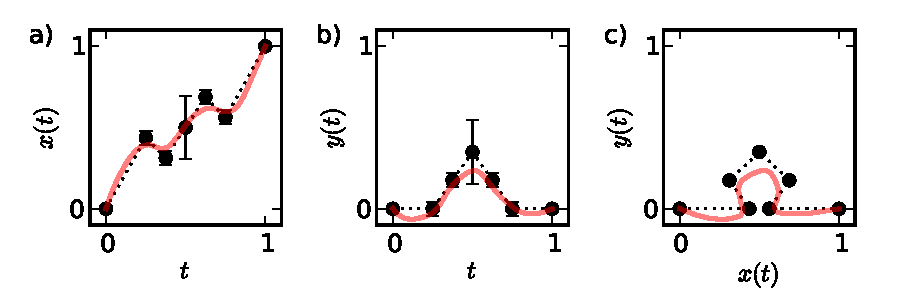
\includegraphics{fig1.pdf}
\caption{Two Gaussian Processes (panel a) for $x(t)$ and panel b) for
  $y(t)$ with \Matern covariance functions and 7 ``observations'' that
  look like a puzzle nub when plotted as a two dimensional function of
  time (panel c).  The GP realizations (solid red lines) show the
  results of choosing good nub-like parameters for the \Matern
  covariance function of $\sigma = 1, \rho = 1.5, \nu = 2$.}
\label{fig:controls}
\end{figure}

Realizing this GP is straightforward with PyMC, requiring little more
than the following code:
\begin{verbatim}
M, C = uninformative_prior_gp(0., diff_degree, amp, scale)
gp.observe(M, C, data.puzzle_t, data.puzzle_x, data.puzzle_V)
GPx = gp.GPSubmodel('GP', M, C, pl.arange(1))
X = GPx.value.f(pl.arange(0., 1.0001, 1. / steps))
\end{verbatim}

By mapping the nubs from these pairs of GPs to the edges of graphs
embedded in the plane, I automatically generated random puzzles (for
example, Fig~\ref{fig:puzzle}).

\begin{figure}

\includegraphics[width=\textwidth]{fig2.pdf}
\caption{A small, randomly generated puzzle, using pairs of Gaussian
  Processes with \Matern covariance functions and 7 ``observations''
  when good nub-like parameters for the \Matern covariance function
  ($\sigma = 1, \rho = 1.5, \nu = 2$) are selected.}
\label{fig:puzzle}
\end{figure}

To explore the effects of the amplitude, scale, and degree of
differentiability parameters, I varied each parameter individually
through a range of values, while holding the other two fixed at good
parameters for puzzle nubs.
 
%%%%%%%%%%%%%%%%%%%%%%%%%%%%
%% Results  %%
%%
%% The Results and Discussion may be combined into a single section or
%% presented separately. Results of statistical analysis should
%% include, where appropriate, relative and absolute risks or risk
%% reductions, and confidence intervals. The results and discussion
%% sections may also be broken into subsections with short,
%% informative headings.

\section*{Results and Discussion}
The results are summarized by Fig~\ref{fig:vary}.
\begin{figure}
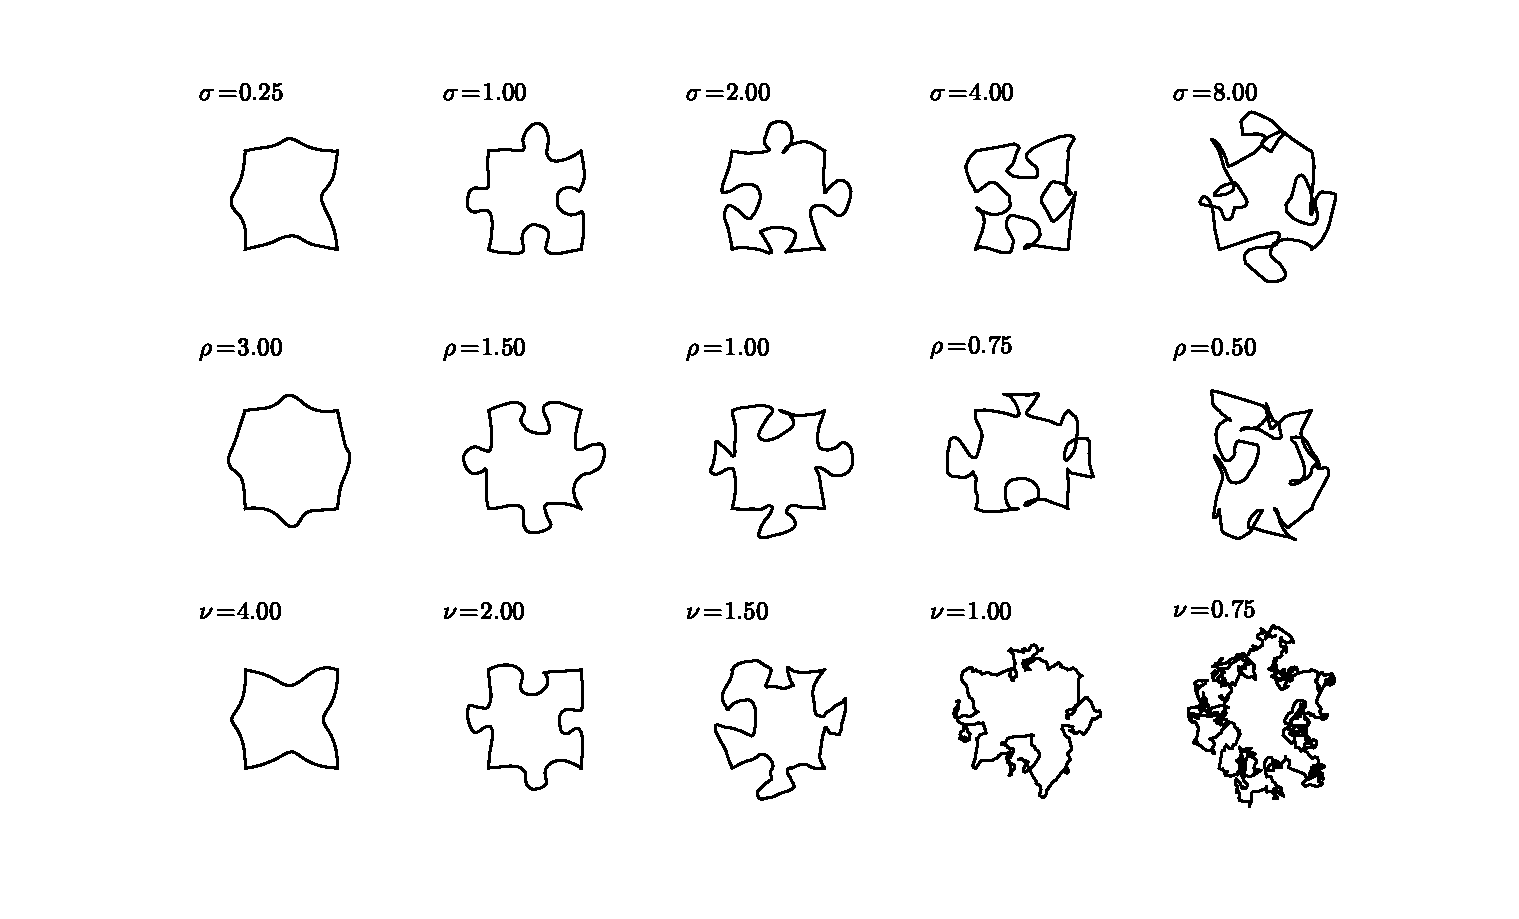
\includegraphics[width=\textwidth]{fig3.pdf}
\caption{Realizations of GP puzzle pieces with varying \Matern
  parameters, using pairs of Gaussian Processes with \Matern
  covariance functions and 7 ``observations''.  The parameters not
  listed in each row are the nub-like parameters $\sigma = 1, \rho =
  1.5,$ and/or $\nu = 2$.}
\label{fig:vary}
\end{figure}

As shown in Fig~\ref{fig:vary}, the \Matern parameters have a complex
interdependence structure, and setting any one incorrectly can lead to
e non-nubby puzzle pieces.  The middle column of the figure shows the
nubby settings, while the entry with $\sigma=.25$ looks qualitatively
very similar to that with $\rho = 3.00$ and also $\nu = 4.00$.

    

%%%%%%%%%%%%%%%%%%%%%%
%% This should state clearly the main conclusions of the research and
%% give a clear explanation of their importance and relevance. Summary
%% illustrations may be included.

\section*{Conclusions}
GPs are an important tool in non-parametric statistics, but be careful
with the parameters, because they have complex interdependencies.


%%%%%%%%%%%%%%%%%%%%%%%%%%%%%%%%
%% A competing interest exists when your interpretation of data or
%% presentation of information may be influenced by your personal or
%% financial relationship with other people or organizations. Authors
%% should disclose any financial competing interests but also any
%% non-financial competing interests that may cause them embarrassment
%% were they to become public after the publication of the manuscript.
%%
%% Authors are required to complete a declaration of competing
%% interests. All competing interests that are declared will be listed
%% at the end of published articles. Where an author gives no
%% competing interests, the listing will read 'The author(s) declare
%% that they have no competing interests'.
%%
%% When completing your declaration, please consider the following
%% questions:
%%
%% Financial competing interests
%%
%% * In the past five years have you received reimbursements, fees,
%%   funding, or salary from an organization that may in any way gain or
%%   lose financially from the publication of this manuscript, either
%%   now or in the future? Is such an organization financing this
%%   manuscript (including the article-processing charge)? If so, please
%%   specify.
%% * Do you hold any stocks or shares in an organization that may in
%%   any way gain or lose financially from the publication of this
%%   manuscript, either now or in the future? If so, please specify.
%% * Do you hold or are you currently applying for any patents
%%   relating to the content of the manuscript? Have you received
%%   reimbursements, fees, funding, or salary from an organization
%%   that holds or has applied for patents relating to the content of
%%   the manuscript? If so, please specify.
%% * Do you have any other financial competing interests? If so,
%%   please specify.
%%
%% Non-financial competing interests
%%
%% * Are there any non-financial competing interests (political,
%%   personal, religious, ideological, academic, intellectual,
%%   commercial or any other) to declare in relation to this
%%   manuscript? If so, please specify.
%%
%% If you are unsure as to whether you or one of your co-authors has a
%% competing interest, please discuss it with the editorial office.

\section*{Competing interests }
The author declares that he has no competing interests.

%%%%%%%%%%%%%%%%%%%%%%%%%%%%%%%%
%% 
%% In order to give appropriate credit to each author of a paper, the
%% individual contributions of authors to the manuscript should be
%% specified in this section.

%% An ``author'' is generally considered to be someone who has made
%% substantive intellectual contributions to a published study. To
%% qualify as an author one should 1) have made substantial
%% contributions to conception and design, or acquisition of data, or
%% analysis and interpretation of data; 2) have been involved in
%% drafting the manuscript or revising it critically for important
%% intellectual content; and 3) have given final approval of the
%% version to be published. Each author should have participated
%% sufficiently in the work to take public responsibility for
%% appropriate portions of the content. Acquisition of funding,
%% collection of data, or general supervision of the research group,
%% alone, does not justify authorship.

%% We suggest the following kind of format (please use initials to
%% refer to each author's contribution): AB carried out the molecular
%% genetic studies, participated in the sequence alignment and drafted
%% the manuscript. JY carried out the immunoassays. MT participated in
%% the sequence alignment. ES participated in the design of the study
%% and performed the statistical analysis. FG conceived of the study,
%% and participated in its design and coordination and helped to draft
%% the manuscript. All authors read and approved the final manuscript.

%% All contributors who do not meet the criteria for authorship should
%% be listed in an acknowledgements section. Examples of those who
%% might be acknowledged include a person who provided purely
%% technical help, writing assistance, or a department chair who
%% provided only general support.

\section*{Authors contributions}
AF designed the study, performed the analysis, and wrote the paper.


    


 
%%%%%%%%%%%%%%%%%%%%%%%%%%%%%%%%%%%%%%%%%%%%%%%%%%%%%%%%%%%%%
%%                  The Bibliography                       %%
%%                                                         %%              
%%  Bmc_article.bst  will be used to                       %%
%%  create a .BBL file for submission, which includes      %%
%%  XML structured for BMC.                                %%
%%                                                         %%
%%                                                         %%
%%  Note that the displayed Bibliography will not          %% 
%%  necessarily be rendered by Latex exactly as specified  %%
%%  in the online Instructions for Authors.                %% 
%%                                                         %%
%%%%%%%%%%%%%%%%%%%%%%%%%%%%%%%%%%%%%%%%%%%%%%%%%%%%%%%%%%%%%


{\ifthenelse{\boolean{publ}}{\footnotesize}{\small}
 \bibliographystyle{bmc_article}  % Style BST file
  \bibliography{bibliography} }     % Bibliography file (usually '*.bib' ) 

%%%%%%%%%%%

\ifthenelse{\boolean{publ}}{\end{multicols}}{}

%%%%%%%%%%%%%%%%%%%%%%%%%%%%%%%%%%%
%%                               %%
%% Additional Files              %%
%%                               %%
%%%%%%%%%%%%%%%%%%%%%%%%%%%%%%%%%%%

\section*{Additional Files}
  \subsection*{Additional file 1 --- Source Code}
    The source code used to generate puzzles and all plots in this paper with the Python PyMC GP Package is available under FLOSS GPL 3.0 Licence from \url{http://github.com/aflaxman/pymc-gp-pzzle}.

\end{bmcformat}
\end{document}







